
\texttt{InferPy} (\cite{cozar2019inferpy}) is a high-level API for probabilistic modeling written in \texttt{Python} and capable of running on top of \texttt{Edward} and \texttt{Tensorflow}. \texttt{InferPy's API} is strongly inspired by \texttt{Keras} and it has a focus on enabling flexible data processing, easy-to-code probablistic modeling, scalable inference and robust model validation.

\begin{figure}[h!]
    \centering
    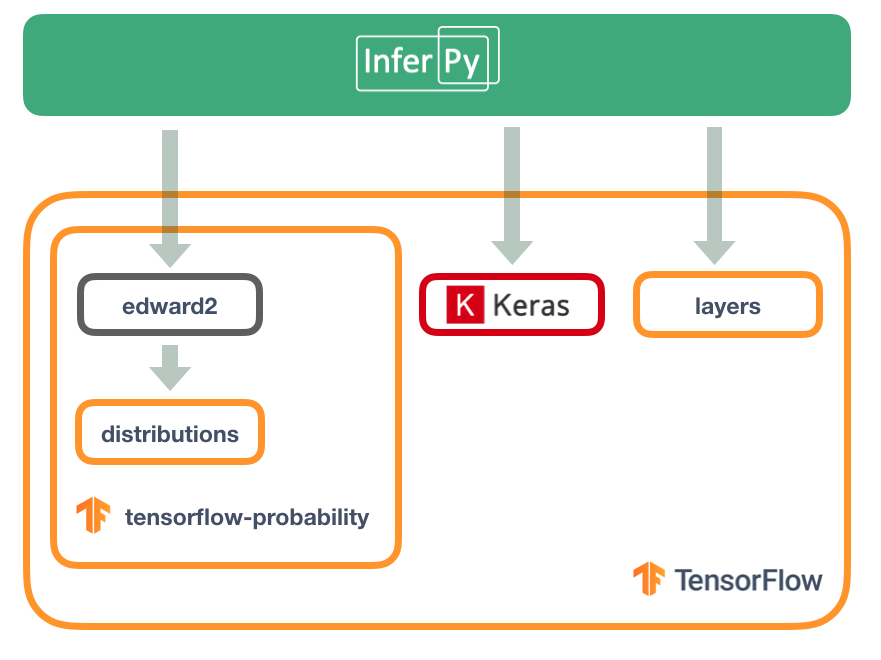
\includegraphics[width=0.7\textwidth]{Chapters/InferPy/arch.png}
    \caption{InferPy architecture.}
\end{figure}

The main features of InferPy are:
\begin{itemize}
    \item Allows a simple definition over probabilistic models containing or not neural networks.
    \item All models that can be defined using \texttt{Edward2} can also be defined in  \texttt{InferPy}, whose probability distributions are mainly inherited from \texttt{tensorflow-probability}.
    \item All the models parameters can be defined using the standard \texttt{Python} types (\texttt{Numpy} compatibility).
    \item \texttt{InferPy} relies on top of \texttt{Edward}'s inference engine, therefore, it includes all the inference algorithms avaible in that package.
    \item An additional advantage of using \texttt{Edward} and \texttt{TensorFlow} as inference engine is that all the parallelization details are hidden to the user. Moreover, the same code will run either in CPUs or GPUs.
\end{itemize}

\section{Installation}

InferPy has the following requirements:
\begin{itemize}
    \item Python \( \geq 3.5 \) and \( < 3.8 \).  
    \item Tensorflow \(\geq  1.12.1 \) and \( < 2.0 \).
    \item Tensorflow-probability \( 0.7.0 \).
    \item NetworkX \( \geq 2.2.0 \) and \( < 3.0 \).   
\end{itemize}

InferPy is available at \texttt{Pip} and can be installed with the following command:

\begin{minted}{sh}
    pip install inferpy
\end{minted}

\section{Usage guide with PCA}

In this section we are constructing a PCA inference model with \texttt{InferPy}. Programming and \texttt{Python} knowledge are assumed, the guidance will be over the API usage.

Let us remember the variables we had in the model, consider \( X_1, \dots, X_N \) i.i.d \( \mathbb{R}^D \) variables, these are the observed ones. Then there are \( Z_1,\dots,Z_N \) hidden variables that correspond to the hidden representation of the data in \( \mathbb{R}^K \). There is also a global hiddel variable \( \bm{W} \) modeling the linear transformation from one space to the other. We are also considering another global variable \( \bm{W}_0 \) that will allow the model to generate non cetered points. 

The hidden variables prior is a centered gaussian and the data is supposed to be generated as
\[
     X_n \mid z_n, \bm{w}, \bm{w_0} \sim \mathcal{N}(\bm{w}^T z_n + \bm{w_0}, I)
\]
No noise is being considered in this example.

\begin{figure}[h!]
    \centering
    \begin{tikzpicture}[
      node distance=1cm and 0.5cm,
      mynode/.style={draw,circle,text width=0.6cm,align=center},
      param/.style={draw,text width=0.5cm,align=center}
      ]
  
      \node[mynode] (theta) {\(\bm{W}\)};
      \node[mynode, below left=of theta] (zn) {\(Z_{n}\)};
      \node[mynode, below right=of theta] (xn) {\(X_{n}\)};
      \node[mynode, above right=of xn] (theta0) {\(\bm{W}_0\)};

  
      \plate{} {(zn)(xn)} {\(n = 1\dots N\)}; %
      \path (theta) edge[-latex] (xn)
      (theta0) edge[-latex] (xn)
      (zn) edge[-latex] (xn)
      ;
  
    \end{tikzpicture}
    \caption{Probabilistic PCA model. No noise considered.}
  \end{figure}
  
  The database we are using is \texttt{Mnist}, which is a largely used dataset on a set of handwritten digits.

  \begin{figure}[h!]
    \centering
    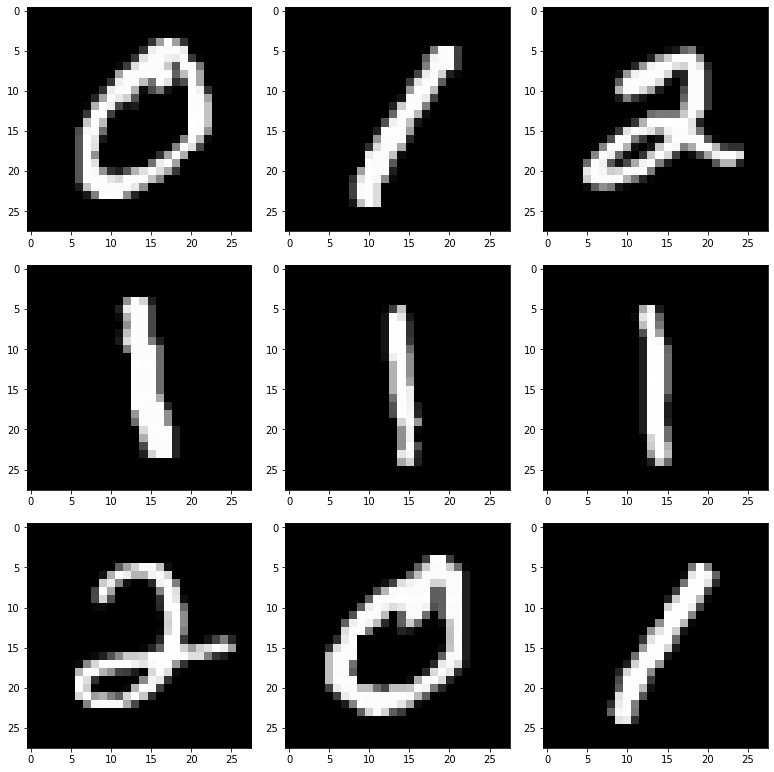
\includegraphics[width=0.5\textwidth]{Chapters/InferPy/mnist.png}
    \caption{Mnist dataset example.}
\end{figure}

The full model definition would be the following:
\begin{minted}[]{python}
    @inf.probmodel
    def pca(k,d):
        w =  inf.Normal(loc=tf.zeros([k,d]),
                       scale=1, name="w")                    # shape = [k,d]
        w0 = inf.Normal(loc=tf.zeros([d]),
                        scale=1, name="w0")                   # shape = [d]
        with inf.datamodel():
            z = inf.Normal(tf.zeros([k]),1, name="z")         # shape = [N,k]
            x = inf.Normal(np.dot(z,w) + w0, 1, name="x")     # shape = [N,d]
\end{minted}

Models are defined as \texttt{Python} functions to which the macro \texttt{@inf.probmodel} must be placed right before. In this case we are defining a model with 2 parameters:

\begin{minted}{python}
    @inf.probmodel
    def pca(k, d):
\end{minted}

Now we declare the global hidden variables, we use the distributions inside \texttt{InferPy} which is assumed to be imported as \texttt{inf}, in this case \texttt{inf.Normal}. This distribution has three arguments, the mean (\texttt{loc}), the variance (\texttt{scale}), and the name of the variable, this last parameter is needed as its how this model and the variational will comunicate.

If either the mean or the variance are given as an array, a constant value on the other parameter would be interpreted as a constant array of the corresponding size.
\begin{minted}[]{python}
    w =  inf.Normal(loc=tf.zeros([k,d]), scale=1, name="w")                   
\end{minted}
Here we are defining a \( K\times D \)  Gaussian distributed variable with mean \( 0 \) and variance \( 1 \), named "w".

We have reached the point where we have to define a set of i.i.d random variables, one for each observation, \texttt{InferPy} gives a explicit sintaxis for this, variables defined inside \texttt{with inf.datamodel(size)} are replicated and i.i.d of each other. The size can be ommited as it is calculated from the dataset.
This is how we declare the hiddel local variables in our model
\begin{minted}[]{python}
    with inf.datamodel():
        z = inf.Normal(tf.zeros([k]),1, name="z")  
\end{minted}

Our generative model is now defined, now we might define the variational one:

\begin{minted}{python}
    @inf.probmodel
    def Q(k,d):
        qw_loc = inf.Parameter(tf.zeros([k,d]), name="qw_loc")
        qw_scale = tf.math.softplus(inf.Parameter(tf.ones([k,d]), name="qw_scale"))
        qw = inf.Normal(qw_loc, qw_scale, name="w")

        qw0_loc = inf.Parameter(tf.ones([d]), name="qw0_loc")
        qw0_scale = tf.math.softplus(inf.Parameter(tf.ones([d]), name="qw0_scale"))
        qw0 = inf.Normal(qw0_loc, qw0_scale, name="w0")
    
        with inf.datamodel():
            qz_loc = inf.Parameter(np.zeros([k]), name="qz_loc")
            qz_scale = tf.math.softplus(inf.Parameter(tf.ones([k]), name="qz_scale"))
            qz = inf.Normal(qz_loc, qz_scale, name="z")
\end{minted}

in this case, among the variables, we must define each parameter. Let us focus on "w". 